\newpage

\section{РАЗРАБОТКА ПРОГРАММЫ}

\subsection{Выбор средств программирования}

Операционная система: \textbf{Ubuntu 20.10}.

Сервер: \textbf{LAMP} - Linux Apache2 MySQL PHP.

Блокнот: \textbf{VS Code 1.52.1}.

Браузер: \textbf{Mozilla Firefox 81.0.2}

\subsubsection*{Установка LAMP}

Перед установкой LAMP обновляем список пакетов, используя команду \textbf{sudo apt update}. Устанавливаем LAMP командой \textbf{sudo apt install apache2 php libapache2-mod-php php-mysql mysql-server phpmyadmin}.
Скриншот терминала на рисунке~\ref{fig:sudo-apt-install-apache2} (стр.~\pageref{fig:sudo-apt-install-apache2}).

\begin{figure}[p]
    \center{
        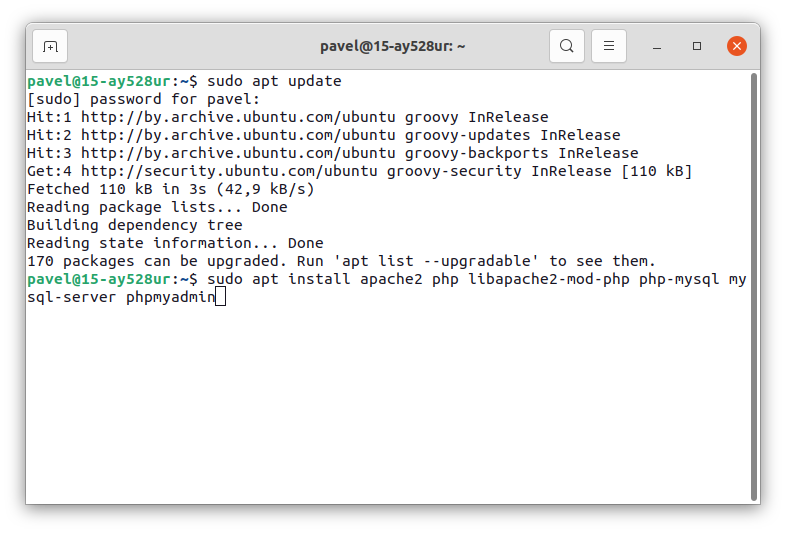
\includegraphics[width=10.5cm]
        {../_input/programDevelopment/install/sudo-apt-install-step-0.png}
    }
    \caption{Установка LAMP}
    \label{fig:sudo-apt-install-apache2}
\end{figure}

При установке пакетов нужно согласиться с скачиванием пакетов и их установкой, нажав на клавишу <<Y>>.
Скриншот терминала на рисунке~\ref{fig:sudo-apt-install-apache2-step-1} (стр.~\pageref{fig:sudo-apt-install-apache2-step-1}).

\begin{figure}[p]
    \center{
        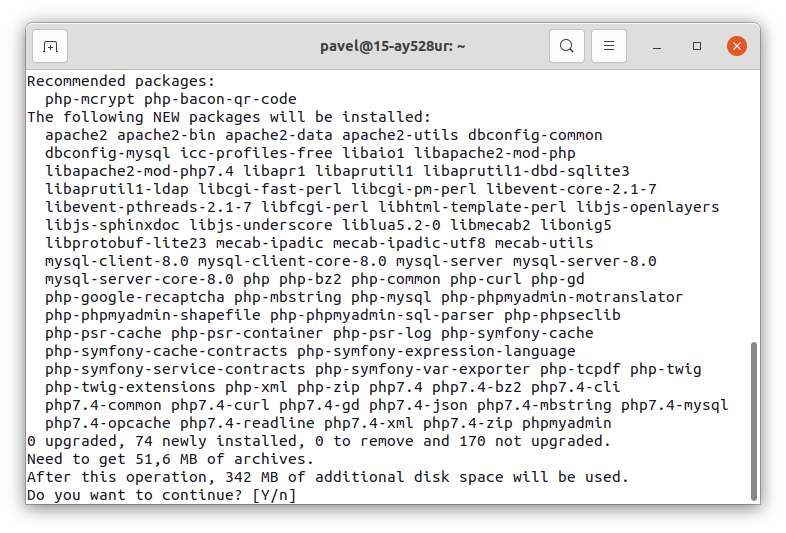
\includegraphics[width=10.5cm]
        {../_input/programDevelopment/install/sudo-apt-install-step-1.png}
    }
    \caption{Согласиться установить LAMP: нажать клавишу <<Y>>}
    \label{fig:sudo-apt-install-apache2-step-1}
\end{figure}

Выбираем флажки при установке, используя клавишу <<пробел>>. После выбранных пунктов родолжаем, нажав клавишу <<Enter>>.
Скриншот терминала на рисунке~\ref{fig:sudo-apt-install-apache2-step-2} (стр.~\pageref{fig:sudo-apt-install-apache2-step-2}).

\begin{figure}[p]
    \center{
        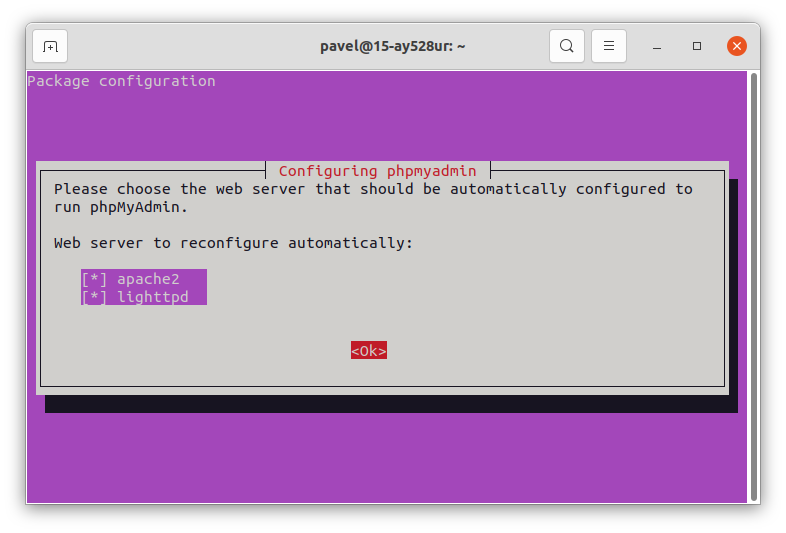
\includegraphics[width=10.5cm]
        {../_input/programDevelopment/install/sudo-apt-install-step-2.png}
    }
    \caption{Выбор флажков того, что установить, при установке LAMP}
    \label{fig:sudo-apt-install-apache2-step-2}
\end{figure}

Отвечаем на вопрос. Нажимаем клавишу <<Enter>> для продолжнения.
Скриншот терминала на рисунке~\ref{fig:sudo-apt-install-apache2-step-3} (стр.~\pageref{fig:sudo-apt-install-apache2-step-3}).

\begin{figure}[p]
    \center{
        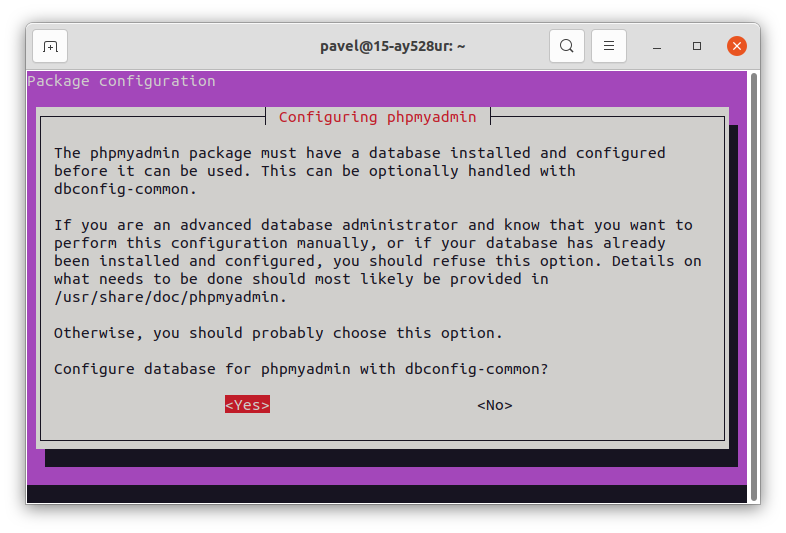
\includegraphics[width=10.5cm]
        {../_input/programDevelopment/install/sudo-apt-install-step-3.png}
    }
    \caption{Вопрос при установке LAMP}
    \label{fig:sudo-apt-install-apache2-step-3}
\end{figure}

После установки пакета <<phpmyadmin>> консоль предложит придумать пароль. Этот пароль будет пользователя под логином <<phpmyadmin>>.
Скриншот терминала на рисунке~\ref{fig:sudo-apt-install-apache2-step-4} (стр.~\pageref{fig:sudo-apt-install-apache2-step-4}).

\begin{figure}[p]
    \center{
        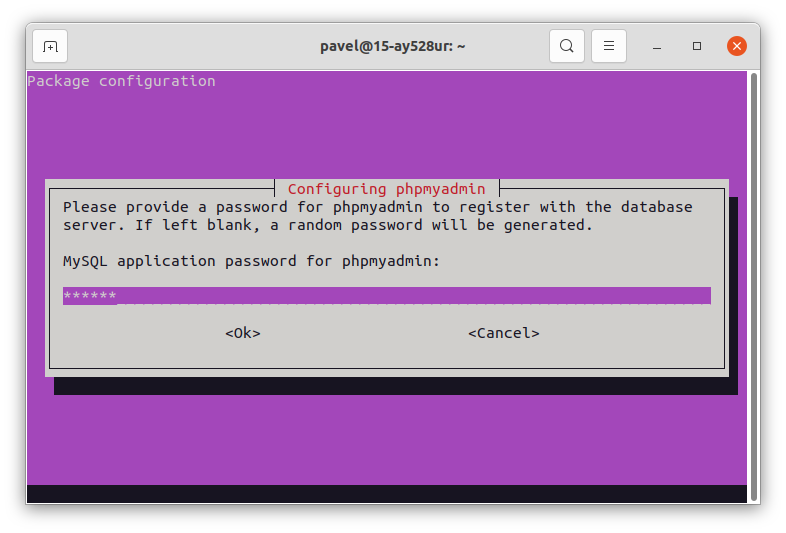
\includegraphics[width=10.5cm]{../_input/programDevelopment/install/sudo-apt-install-step-4.png}
    }
    \caption{Придумываем пароль для пользователя под логином <<phpmyadmin>>}
    \label{fig:sudo-apt-install-apache2-step-4}
\end{figure}

Как придумали пароль для <<phpmyadmin>>, то его нужно повторить. Повторяем пароль.
Скришнот терминала на рисунке~\ref{fig:sudo-apt-install-apache2-step-5} (стр.~\pageref{fig:sudo-apt-install-apache2-step-5}).

\begin{figure}[p]
    \center{
        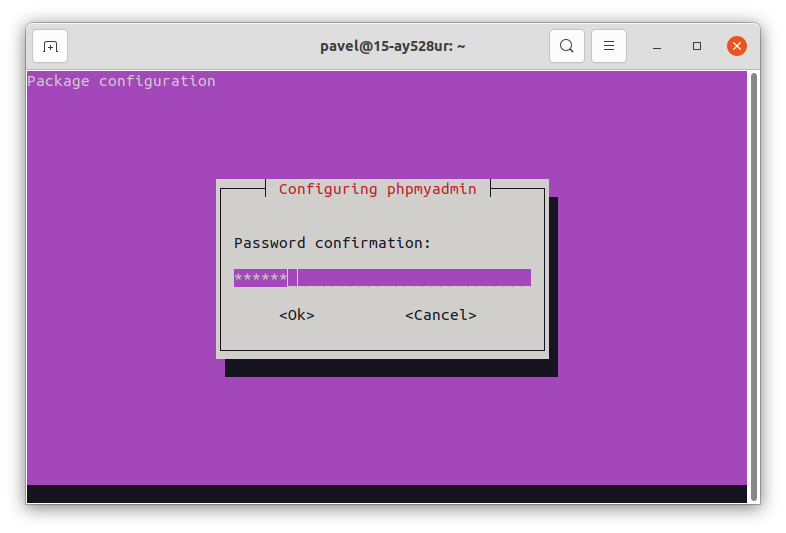
\includegraphics[width=10.5cm]{../_input/programDevelopment/install/sudo-apt-install-step-5.png}
    }
    \caption{Повторяем пароль для пользователя под логином <<phpmyadmin>>}
    \label{fig:sudo-apt-install-apache2-step-5}
\end{figure}

Успешно завершили установку.
Скришнот терминала на рисунке~\ref{fig:sudo-apt-install-apache2-step-6} (стр.~\pageref{fig:sudo-apt-install-apache2-step-6}).

\begin{figure}[p]
    \center{
        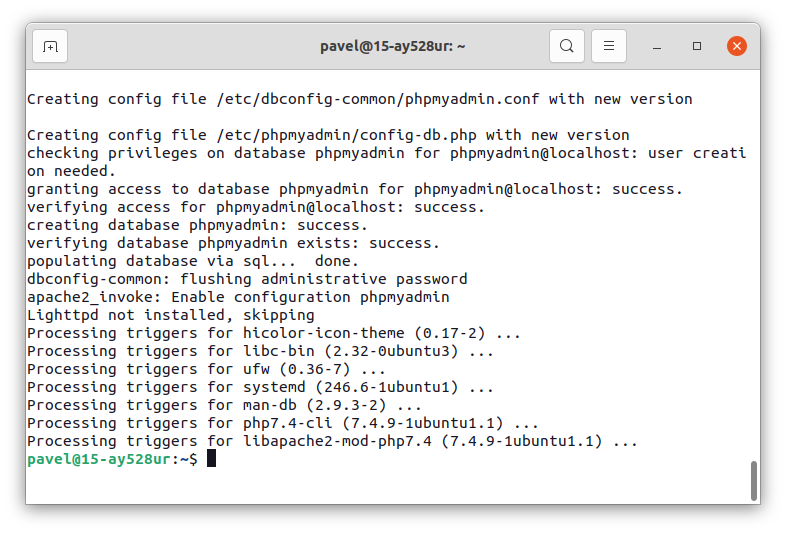
\includegraphics[width=10.5cm]{../_input/programDevelopment/install/sudo-apt-install-step-6.png}
    }
    \caption{Конец устаноки LAMP}
    \label{fig:sudo-apt-install-apache2-step-6}
\end{figure}

После установки Apache2, можем проверить сайт, вписав \textbf{localhost} в адресную строку браузера.
Скриншот браузера с открытым сайтом на рисунке~\ref{fig:sudo-apt-install-apache2-step-7} (стр.~\pageref{fig:sudo-apt-install-apache2-step-7}).

\begin{figure}[p]
    \center{
        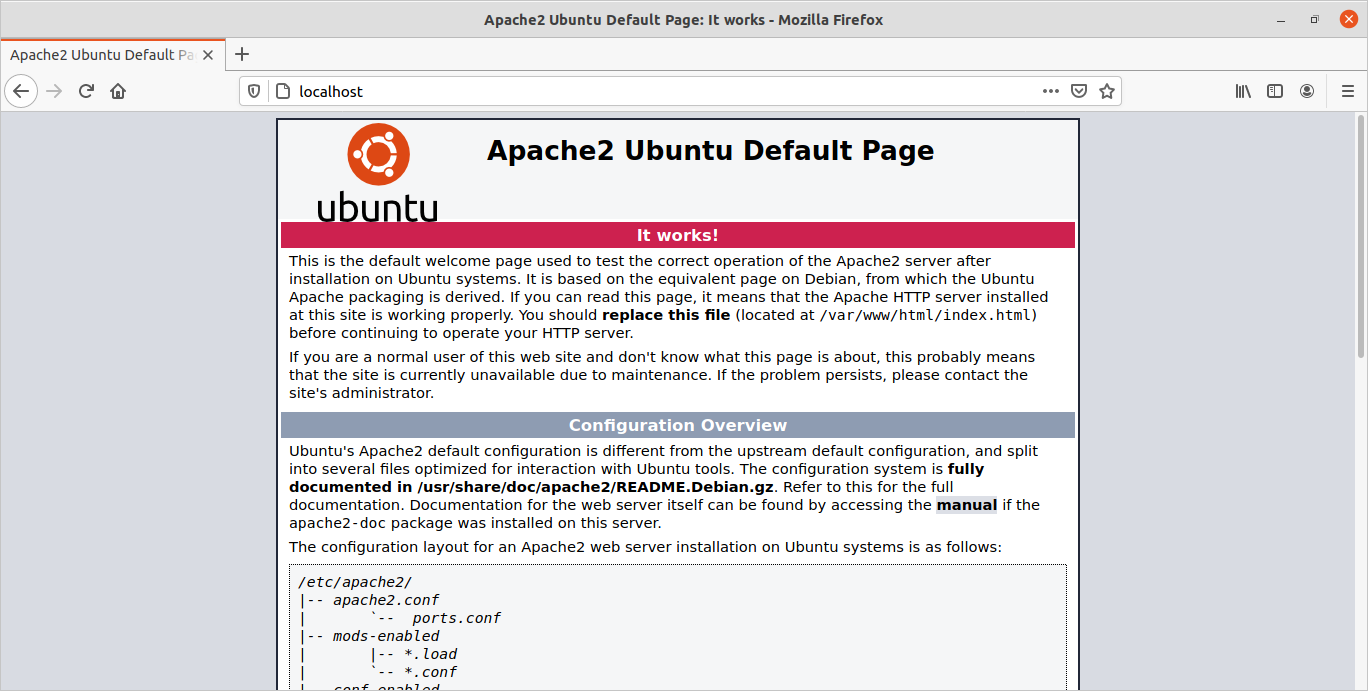
\includegraphics[width=10.5cm]{../_input/programDevelopment/install/sudo-apt-install-step-7.png}
    }
    \caption{Открываем сайт localhost в браузере}
    \label{fig:sudo-apt-install-apache2-step-7}
\end{figure}

\newpage

% = = = = =

\subsubsection*{Создание нового пользователя <<phpmyadmin>> с полными правами доступа}

Заходим на сраницу <<\textbf{localhost/phpmyadmin}>> под логином <<phpmyadmin>> и придуманым паролем: <<222222>> - и видем, что мы не можем создавать базы данных. Создадим пользователя с такими правами. Вводим команду \textbf{sudo mysql -u root -p}. Далее вводим пароль от супер пользователя <<pavel>> нашей системы. Далее вводим придуманный пароль <<222222>> для нашего <<phpmyadmin>>.
Скриншот терминала на рисунке~\ref{fig:make-phpmyadmin-superuser-step-0} (стр.~\pageref{fig:make-phpmyadmin-superuser-step-0}).

\begin{figure}[p]
    \center{
        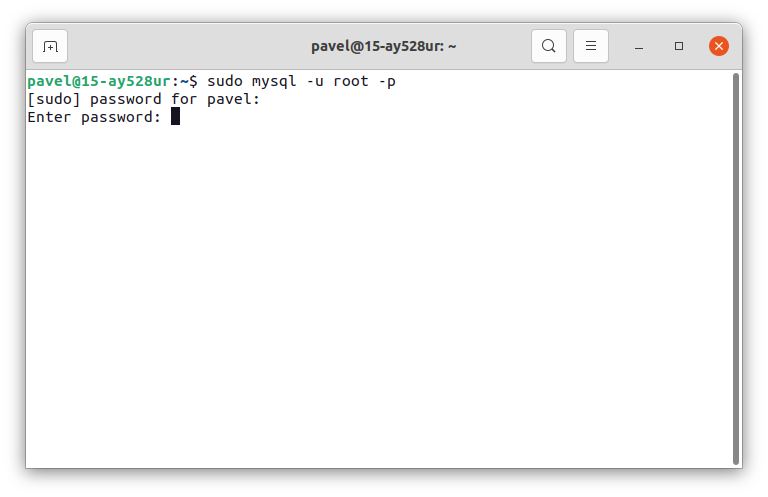
\includegraphics[width=10.5cm]{../_input/programDevelopment/make-phpmyadmin-superuser/make-user-step-0.png}
    }
    \caption{Входим в среду ввода скриптов MySQL}
    \label{fig:make-phpmyadmin-superuser-step-0}
\end{figure}

Теперь мы можем вводить скрипты на языкы MySQL.
Скриншот терминала на рисунке~\ref{fig:make-phpmyadmin-superuser-step-1} (стр.~\pageref{fig:make-phpmyadmin-superuser-step-1}).

\begin{figure}[p]
    \center{
        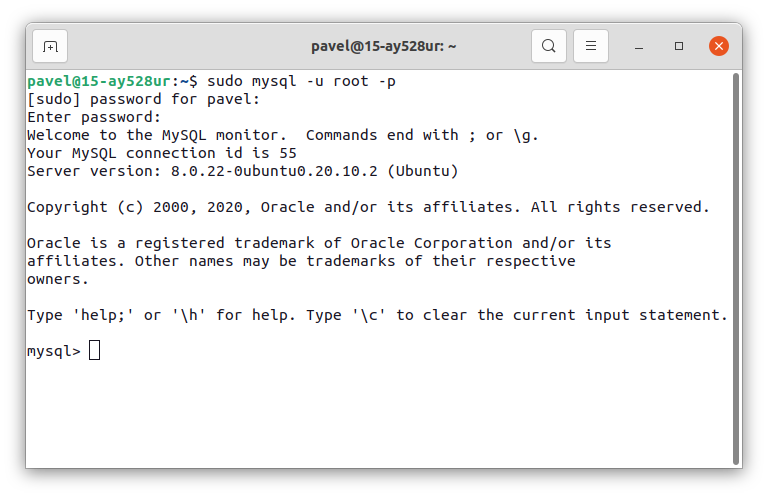
\includegraphics[width=10.5cm]{../_input/programDevelopment/make-phpmyadmin-superuser/make-user-step-1.png}
    }
    \caption{Среда ввода скриптов MySQL}
    \label{fig:make-phpmyadmin-superuser-step-1}
\end{figure}

Создаем пользователя <<admin>> с паролем <<333333>> с помощью команды \textbf{CREATE USER 'admin'@'localhost' IDENTIFIED BY '333333';}.
Скриншот терминала на рисунке~\ref{fig:make-phpmyadmin-superuser-step-2} (стр.~\pageref{fig:make-phpmyadmin-superuser-step-2}).

\begin{figure}[p]
    \center{
        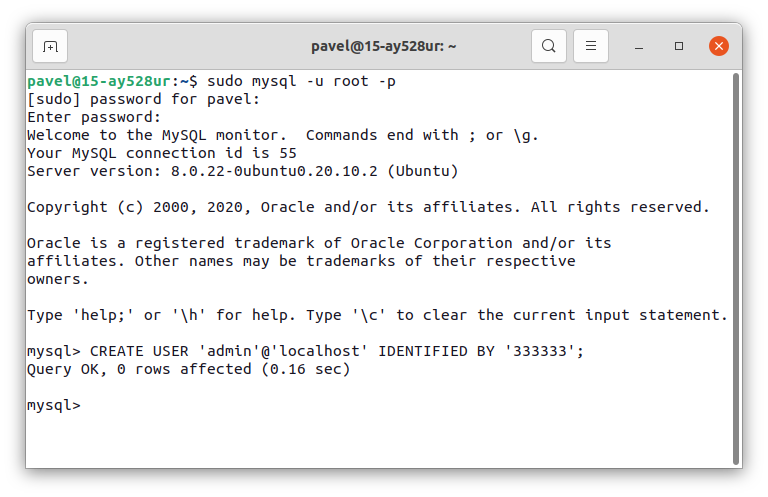
\includegraphics[width=10.5cm]{../_input/programDevelopment/make-phpmyadmin-superuser/make-user-step-2.png}
    }
    \caption{Создаем пользователя и пароль с помощью скрипта}
    \label{fig:make-phpmyadmin-superuser-step-2}
\end{figure}

Выдаем пользователю <<admin>> все права с помощью команды \sloppy \textbf{GRANT ALL PRIVILEGES ON *.* TO 'admin'@'localhost' WITH GRANT OPTION;}.
Скриншот терминала на рисунке~\ref{fig:make-phpmyadmin-superuser-step-3} (стр.~\pageref{fig:make-phpmyadmin-superuser-step-3}).

\begin{figure}[p]
    \center{
        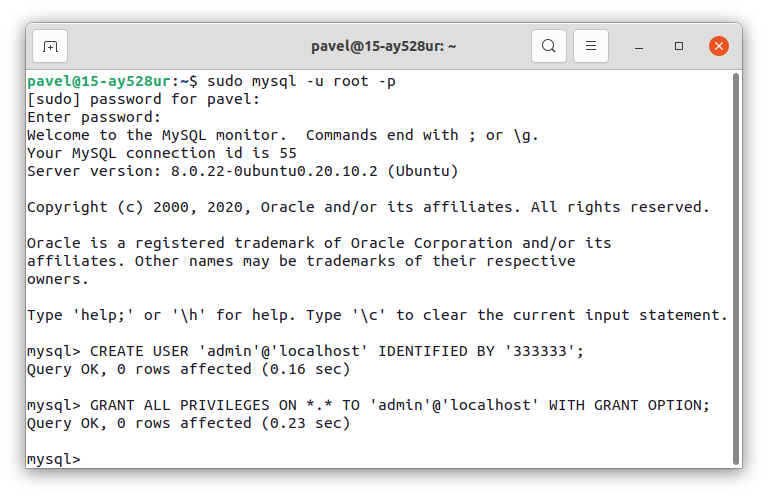
\includegraphics[width=10.5cm]{../_input/programDevelopment/make-phpmyadmin-superuser/make-user-step-3.png}
    }
    \caption{Выдаем права пользователю с помощью скрипта}
    \label{fig:make-phpmyadmin-superuser-step-3}
\end{figure}

Перезагрузим талицы предоставления с компощью команды \textbf{FLUSH PRIVILEGES;}.
Скриншот терминала на рисунке~\ref{fig:make-phpmyadmin-superuser-step-4} (стр.~\pageref{fig:make-phpmyadmin-superuser-step-4}).

\begin{figure}[p]
    \center{
        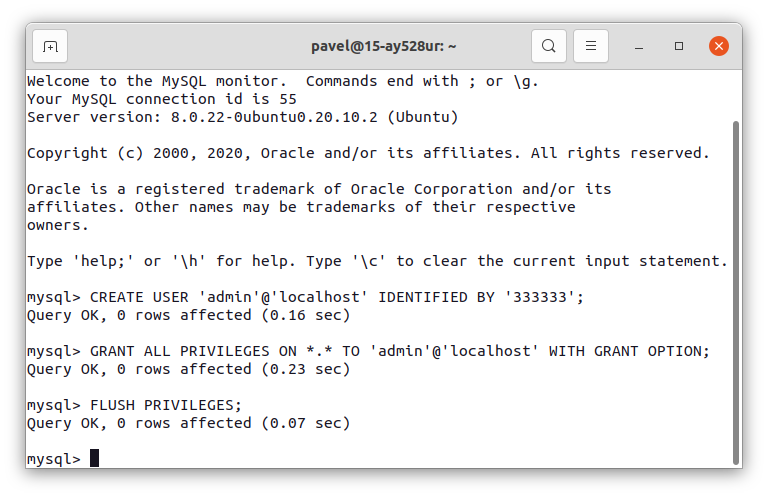
\includegraphics[width=10.5cm]{../_input/programDevelopment/make-phpmyadmin-superuser/make-user-step-4.png}
    }
    \caption{Перезагружаем таблицу предоставления}
    \label{fig:make-phpmyadmin-superuser-step-4}
\end{figure}

Закрываем ввод MySQL скриптов с помощью команды \textbf{exit}.
Скриншот терминала на рисунке~\ref{fig:make-phpmyadmin-superuser-step-5} (стр.~\pageref{fig:make-phpmyadmin-superuser-step-5}).

\begin{figure}[p]
    \center{
        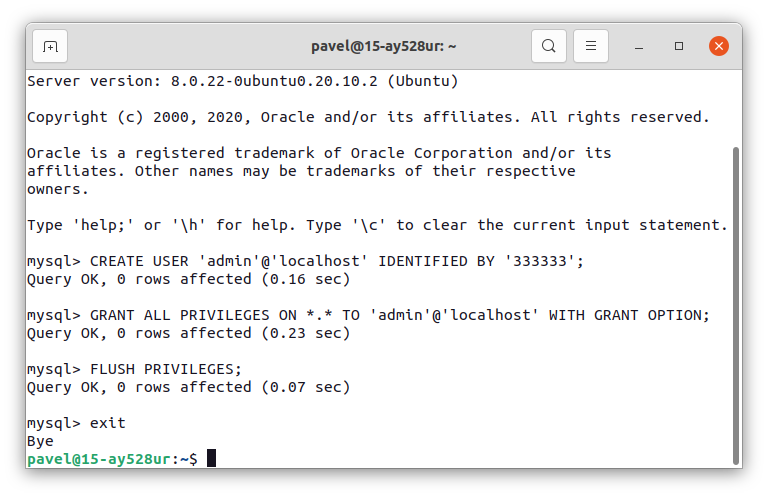
\includegraphics[width=10.5cm]{../_input/programDevelopment/make-phpmyadmin-superuser/make-user-step-5.png}
    }
    \caption{Закрываем среду MySQL}
    \label{fig:make-phpmyadmin-superuser-step-5}
\end{figure}

Заходим на сраницу <<\textbf{localhost/phpmyadmin}>> под логином <<admin>> и паролем <<333333>>. 
Скриншот браузера на рисунке~\ref{fig:make-phpmyadmin-superuser-step-6} (стр.~\pageref{fig:make-phpmyadmin-superuser-step-6}).

\begin{figure}[p]
    \center{
        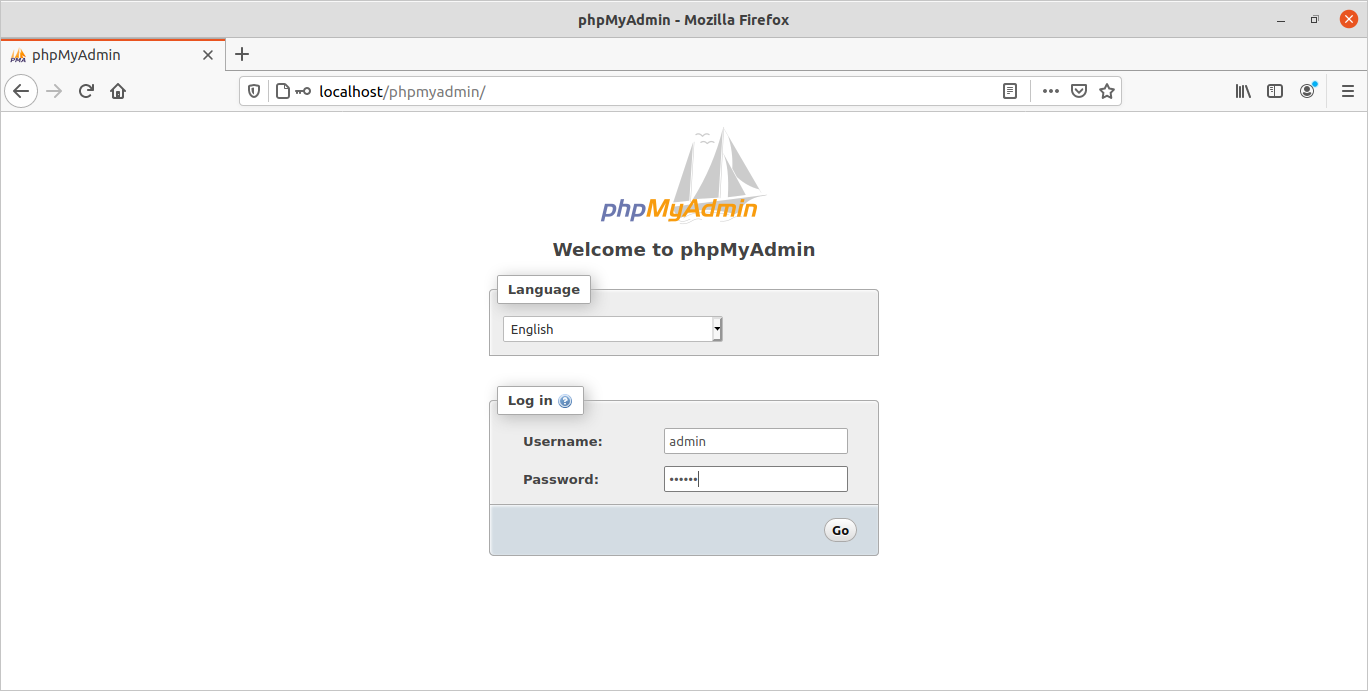
\includegraphics[width=10.5cm]{../_input/programDevelopment/make-phpmyadmin-superuser/make-user-step-6.png}
    }
    \caption{Страница <<localhost/phpmyadmin>>}
    \label{fig:make-phpmyadmin-superuser-step-6}
\end{figure}

Теперь можем создавать базу данных.
Скриншот браузера на рисунке~\ref{fig:make-phpmyadmin-superuser-step-7} (стр.~\pageref{fig:make-phpmyadmin-superuser-step-7}).

\begin{figure}[p]
    \center{
        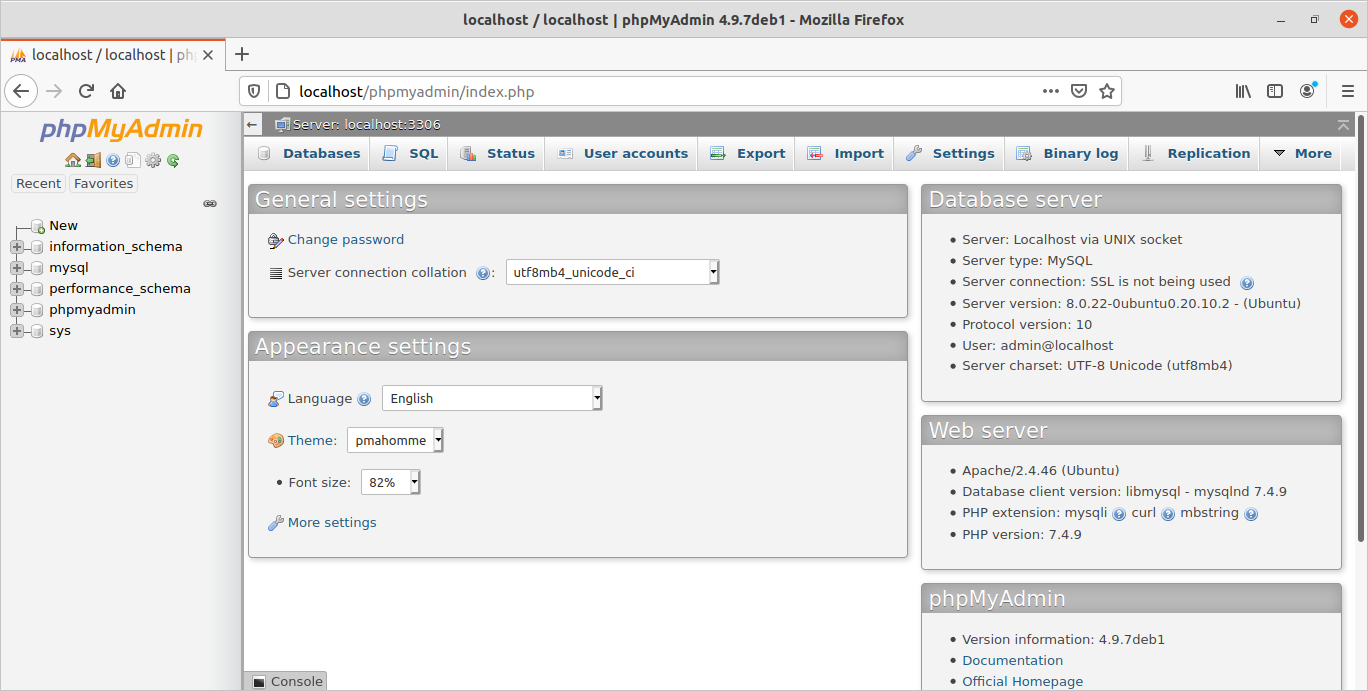
\includegraphics[width=10.5cm]{../_input/programDevelopment/make-phpmyadmin-superuser/make-user-step-7.png}
    }
    \caption{Залогиненный пользователь <<admin>> в <<phpmyadmin>>}
    \label{fig:make-phpmyadmin-superuser-step-7}
\end{figure}

\newpage

% = = = = =

\subsubsection*{Выделяем свой домен}

Создаем директорию для сайта. Выполняем команду \textbf{sudo mkdir /var/www/mysite}.
Скриншот терминала на рисунке~\ref{fig:sudo-mkdir-mysite} (стр.~\pageref{fig:sudo-mkdir-mysite}).

\begin{figure}[p]
    \center{
        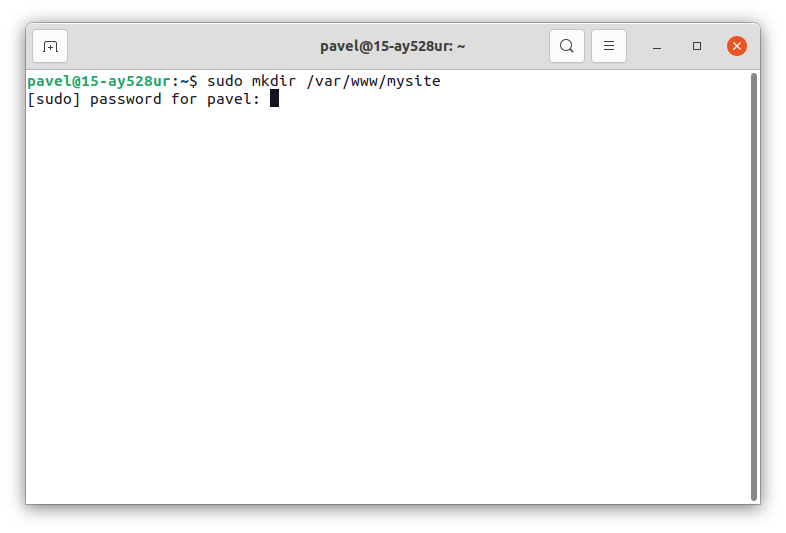
\includegraphics[width=10.5cm]{../_input/programDevelopment/makeDomain/sudo-mkdir-mysite.png}
    }
    \caption{Создаем папку mysite через терминал}
    \label{fig:sudo-mkdir-mysite}
\end{figure}

Так как папка создана через sudo, то изменять её можно только через sudo (под правами суперпользователя). Чтобы мог её изменять обычный пользователь, то нужно выдать ему права. Выдадим права командой \textbf{sudo chown -R \$USER:\$USER /var/www/mysite} (или \textbf{sudo chmod 0777 -R /var/www/mysite}).
Скриншот терминала на рисунке~\ref{fig:sudo-chown} (стр.~\pageref{fig:sudo-chown}).

\begin{figure}[p]
    \center{
        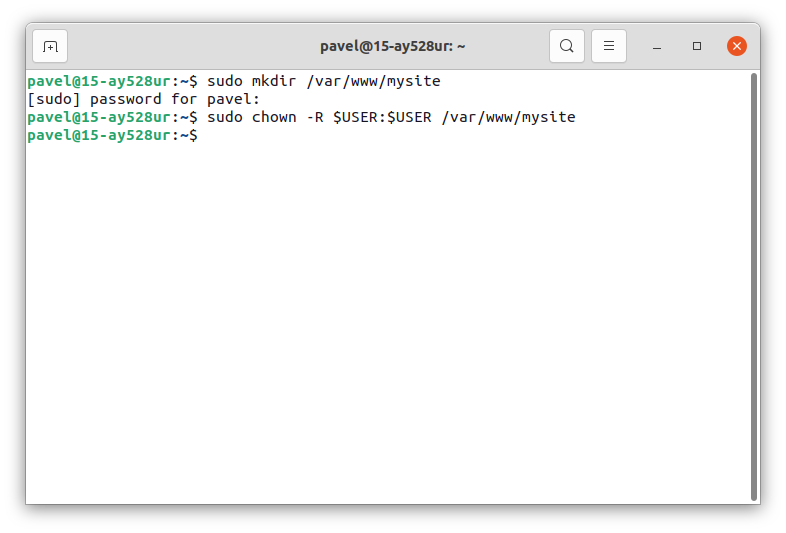
\includegraphics[width=10.5cm]{../_input/programDevelopment/makeDomain/sudo-chown.png}
    }
    \caption{Выдаем права на редактирование}
    \label{fig:sudo-chown}
\end{figure}

Копируем стандартный файл настроек. Выполняем команду \textbf{sudo cp /etc/apache2/sites-available/000-default.conf /etc/apache2/sites-available/mysite.conf}.
Скриншот терминала на рисунке~\ref{fig:sudo-cp-mysite-conf} (стр.~\pageref{fig:sudo-cp-mysite-conf}).

\begin{figure}[p]
    \center{
        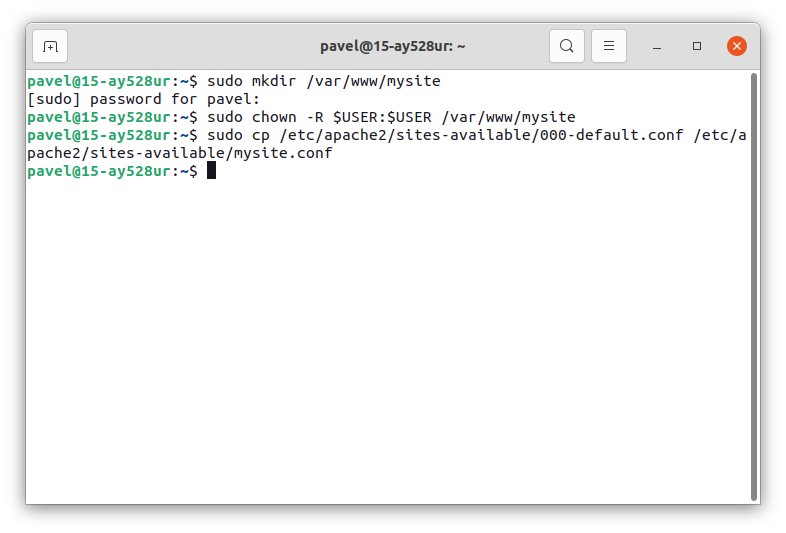
\includegraphics[width=10.5cm]{../_input/programDevelopment/makeDomain/sudo-cp-mysite-conf.png}
    }
    \caption{Копируем стандартный файл настроек}
    \label{fig:sudo-cp-mysite-conf}
\end{figure}

Открываем файл <<mysite.conf>> в редакторе nano. Используем команду \textbf{sudo nano /etc/apache2/sites-available/mysite.conf}.
Скриншот терминала на рисунке~\ref{fig:sudo-nano-mysite-conf} (стр.~\pageref{fig:sudo-nano-mysite-conf}).
Файл <<mysite.conf>> открывается в редакторе nano.
Скриншот терминала на рисунке~\ref{fig:sudo-nano-mysite-conf-step-1} (стр.~\pageref{fig:sudo-nano-mysite-conf-step-1}).

\begin{figure}[p]
    \center{
        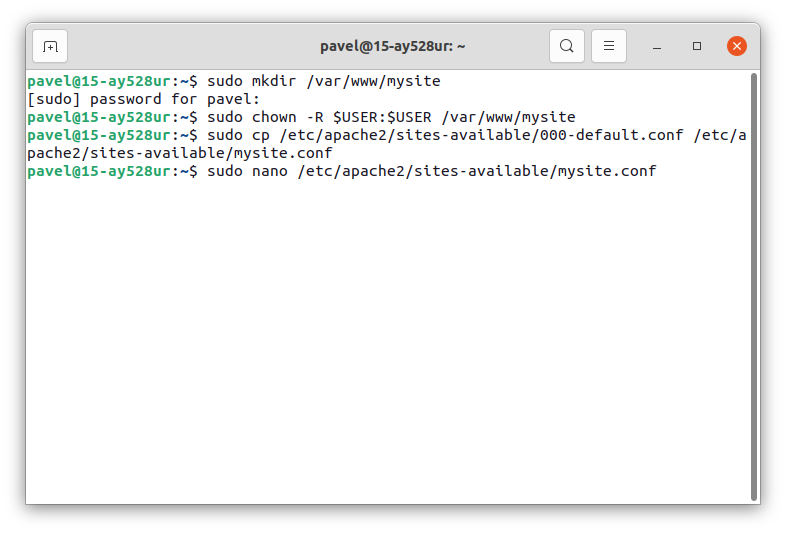
\includegraphics[width=10.5cm]{../_input/programDevelopment/makeDomain/sudo-nano-mysite-conf.png}
    }
    \caption{Открываем файл <<mysite.conf>> в редакторе nano}
    \label{fig:sudo-nano-mysite-conf}
\end{figure}

\begin{figure}[p]
    \center{
        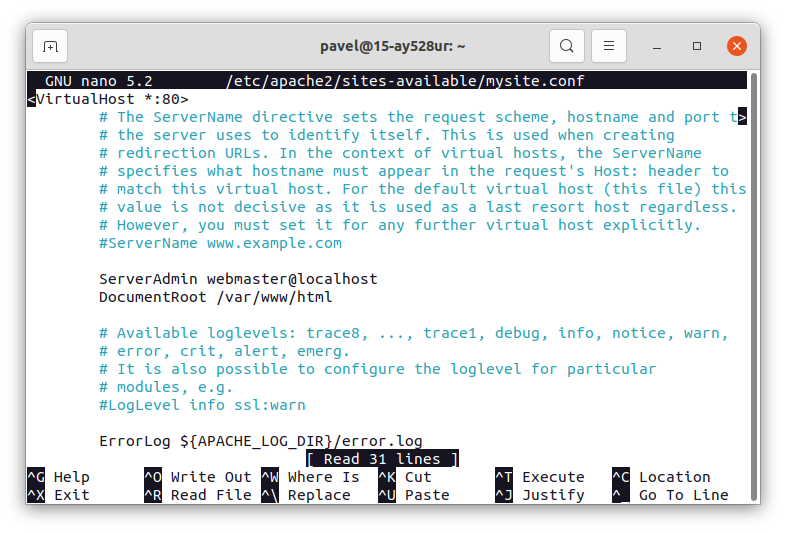
\includegraphics[width=10.5cm]{../_input/programDevelopment/makeDomain/sudo-nano-mysite-conf-step-1.png}
    }
    \caption{Файл <<mysite.conf>> в редакторе nano}
    \label{fig:sudo-nano-mysite-conf-step-1}
\end{figure}

В файле <<mysite.conf>> добавляем строчку <<\textbf{ServarName mysite}>>, который говорит, под каким доменом использовать, то есть в браузере в адрессную строку вводим <<\textbf{mysite}>>. В файле <<mysite.conf>> добавляем строчку <<\textbf{DocumentRoot /var/www/mysite/src}>>, которая говорит, где находятся файлы ресурсов сайта, то есть главный файл <<index.html/index.php>> находится в каталоге <<\textbf{DocumentRoot /var/www/mysite/src}>>.
Скриншот терминала с добавленными строчками на рисунке~\ref{fig:sudo-nano-mysite-conf-step-2} (стр.~\pageref{fig:sudo-nano-mysite-conf-step-2}).
Для сохранения нужно нажать клавишу <<Ctrl>> + <<X>>. Затем нажать клавишу <<Y>>.
Скриншот терминала на рисунке~\ref{fig:sudo-nano-mysite-conf-step-3} (стр.~\pageref{fig:sudo-nano-mysite-conf-step-3}).
Затем нажимаем клавишу <<Enter>>.
Скриншот терминала на рисунке~\ref{fig:sudo-nano-mysite-conf-step-4} (стр.~\pageref{fig:sudo-nano-mysite-conf-step-4}).
В итоге сохранили файл.

\begin{figure}[p]
    \center{
        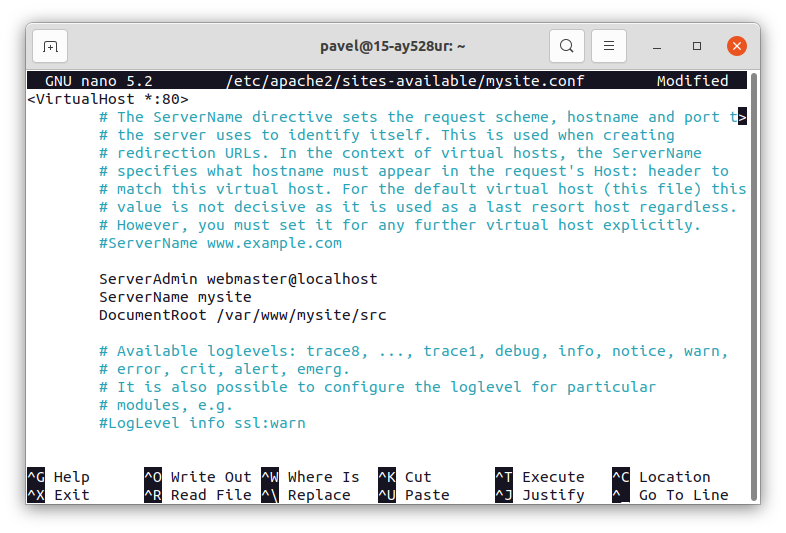
\includegraphics[width=10.5cm]{../_input/programDevelopment/makeDomain/sudo-nano-mysite-conf-step-2.png}
    }
    \caption{Добавляем строчки ServerName, DocumentRoot}
    \label{fig:sudo-nano-mysite-conf-step-2}
\end{figure}

\begin{figure}[p]
    \center{
        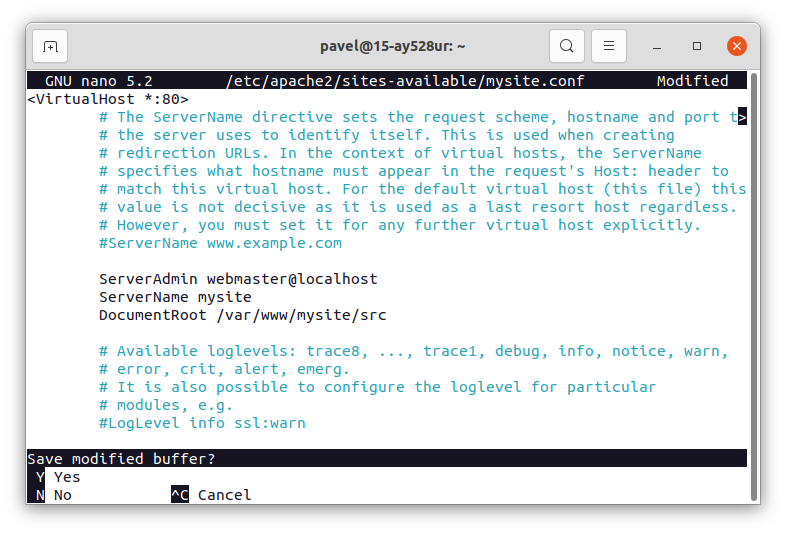
\includegraphics[width=10.5cm]{../_input/programDevelopment/makeDomain/sudo-nano-mysite-conf-step-3.png}
    }
    \caption{Нажимае клавишу <<Ctrl>> + <<X>>, затем <<Y>>}
    \label{fig:sudo-nano-mysite-conf-step-3}
\end{figure}

\begin{figure}[p]
    \center{
        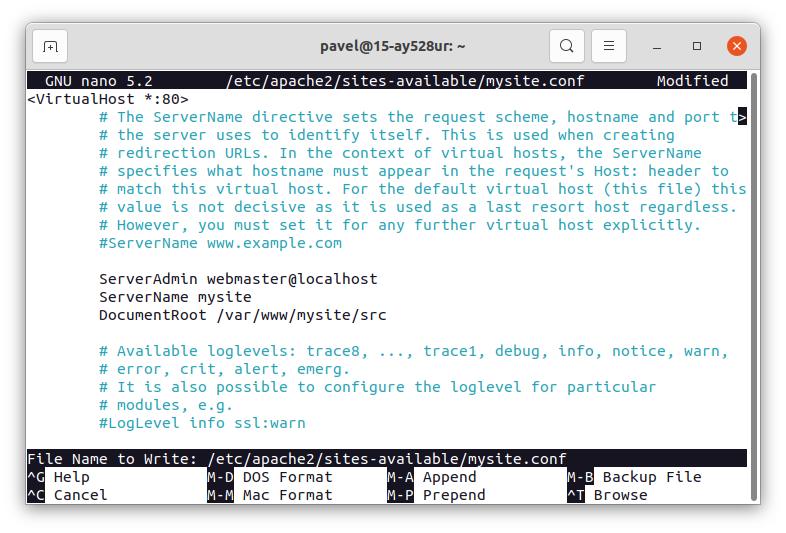
\includegraphics[width=10.5cm]{../_input/programDevelopment/makeDomain/sudo-nano-mysite-conf-step-4.png}
    }
    \caption{Нажали клавишу <<Y>>, затем жмем <<Enter>>}
    \label{fig:sudo-nano-mysite-conf-step-4}
\end{figure}

Применяем настройки, используя команду \textbf{sudo a2ensite mysite}.
Скриншот терминала на рисунке~\ref{fig:sudo-a2ensite} (стр.~\pageref{fig:sudo-a2ensite}).

\begin{figure}[p]
    \center{
        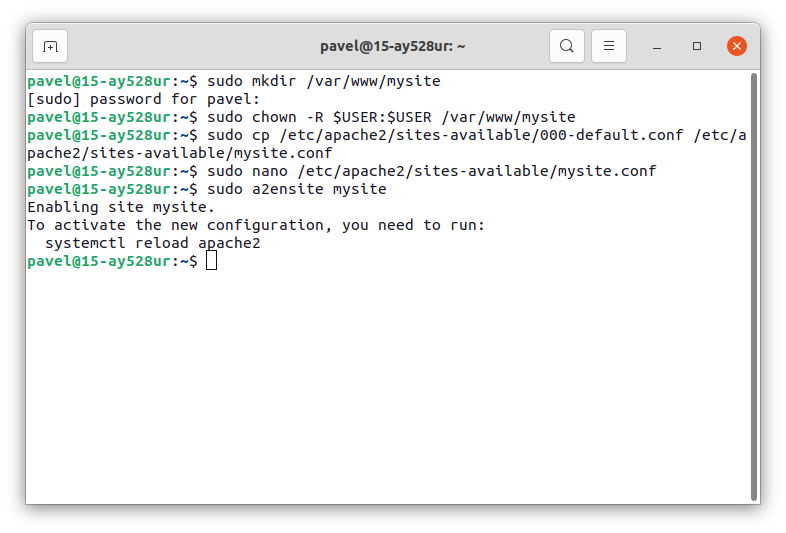
\includegraphics[width=10.5cm]{../_input/programDevelopment/makeDomain/sudo-a2ensite.png}
    }
    \caption{Применяем настройки Apache2}
    \label{fig:sudo-a2ensite}
\end{figure}

Перезагружаем Apache2, используя команду \textbf{sudo systemctl reload apache2}.
Скриншот терминала на рисунке~\ref{fig:sudo-system-ctl-reload-apache2} (стр.~\pageref{fig:sudo-system-ctl-reload-apache2}).

\begin{figure}[p]
    \center{
        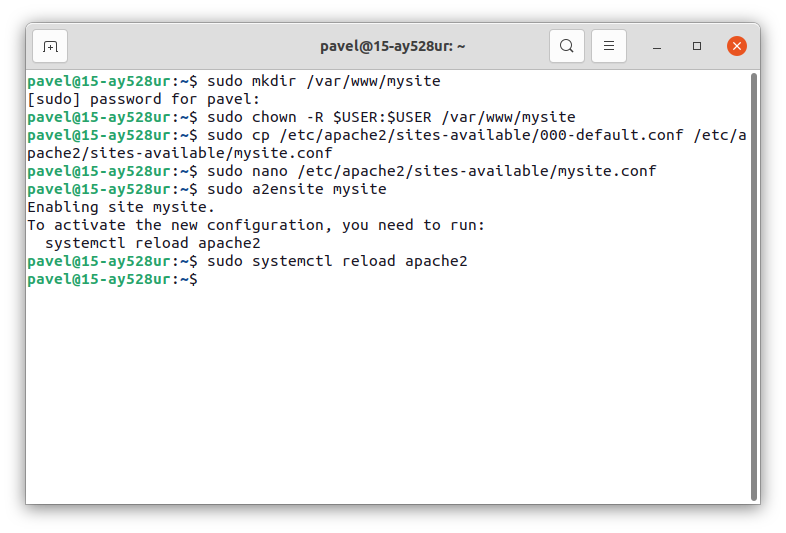
\includegraphics[width=10.5cm]{../_input/programDevelopment/makeDomain/sudo-system-ctl-reload-apache2.png}
    }
    \caption{Применяем настройки Apache2}
    \label{fig:sudo-system-ctl-reload-apache2}
\end{figure}

Если открыть браузер и ввести в адресную строку <<mysite>>, то сайт не откроется.
Его нужно прописать в файле hosts, после чего по адресу <<mysite>> он должен открываться.
Открываем файл <<hosts>> в редакторе nano, используя команду \textbf{sudo nano /etc/hosts}.
Скриншот терминала на рисунке~\ref{fig:sudo-nano-hosts} (стр.~\pageref{fig:sudo-nano-hosts}).
Открылся файл <<hosts>> в редакторе nano.
Скриншот терминала на рисунке~\ref{fig:sudo-nano-hosts-step-1} (стр.~\pageref{fig:sudo-nano-hosts-step-1}).
Добавляем строчку \textbf{127.0.0.1 mysite}.
Скриншот терминала на рисунке~\ref{fig:sudo-nano-hosts-step-2} (стр.~\pageref{fig:sudo-nano-hosts-step-2}).
Для сохранения жмём <<Ctrl>> + <<X>>, затем жмём <<Y>>.
Скриншот терминала на рисунке~\ref{fig:sudo-nano-hosts-step-3} (стр.~\pageref{fig:sudo-nano-hosts-step-3}).
После нажатия <<Y>>, жмем <<Enter>>.
Скриншот терминала на рисунке~\ref{fig:sudo-nano-hosts-step-4} (стр.~\pageref{fig:sudo-nano-hosts-step-4}).
Файл сохранился.

\begin{figure}[p]
    \center{
        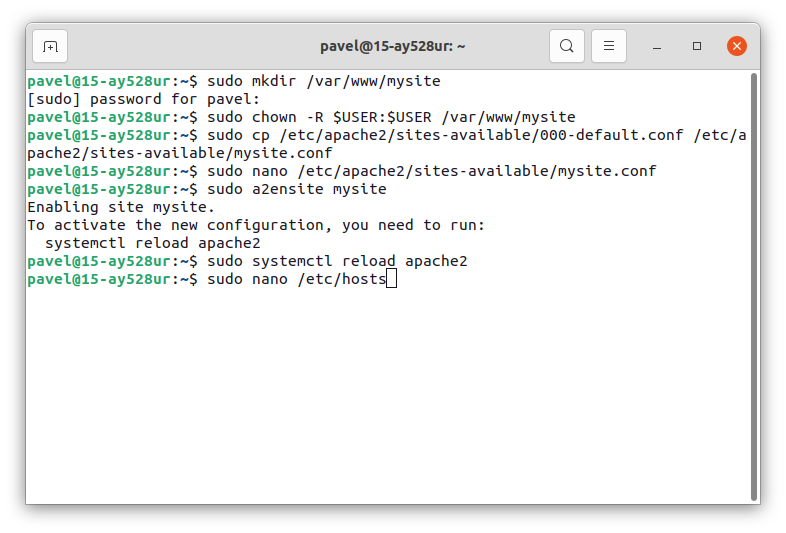
\includegraphics[width=10.5cm]{../_input/programDevelopment/makeDomain/sudo-nano-hosts.png}
    }
    \caption{Открываем файл <<hosts>> в редакторе nano}
    \label{fig:sudo-nano-hosts}
\end{figure}

\begin{figure}[p]
    \center{
        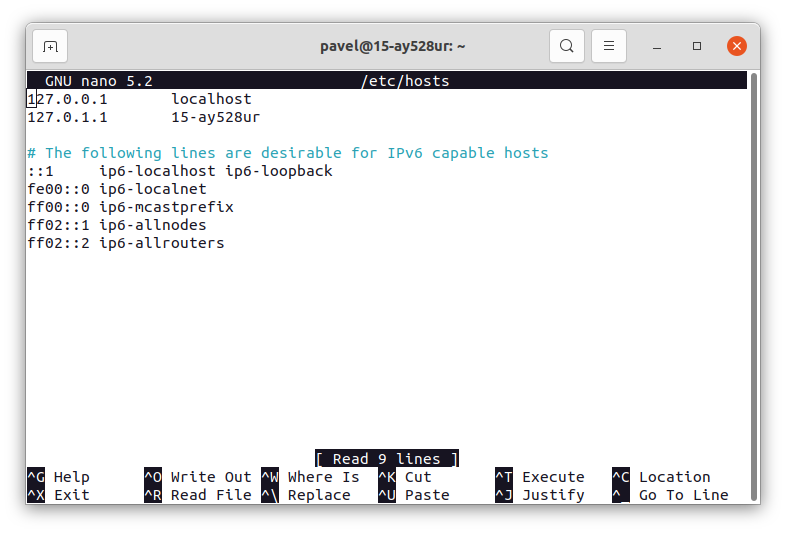
\includegraphics[width=10.5cm]{../_input/programDevelopment/makeDomain/sudo-nano-hosts-step-1.png}
    }
    \caption{Файл <<hosts>> в редакторе nano}
    \label{fig:sudo-nano-hosts-step-1}
\end{figure}

\begin{figure}[p]
    \center{
        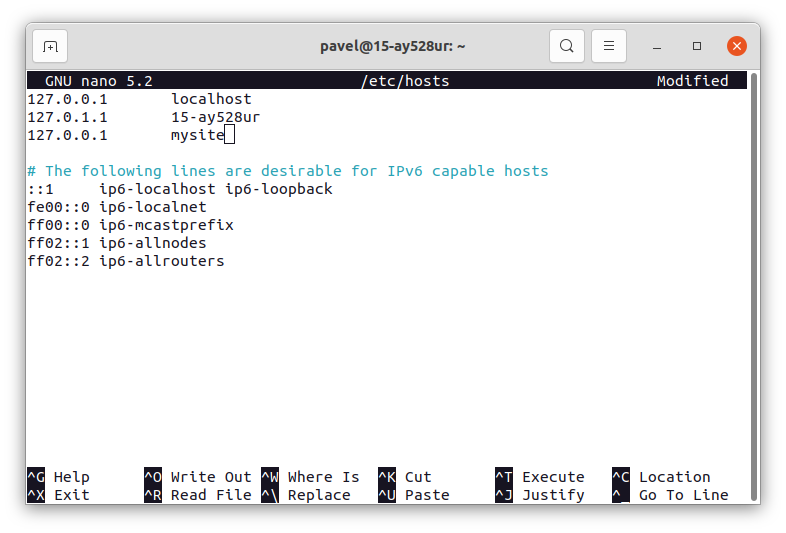
\includegraphics[width=10.5cm]{../_input/programDevelopment/makeDomain/sudo-nano-hosts-step-2.png}
    }
    \caption{Добавляем строчку с доменом <<mysite>> в файле <<hosts>>}
    \label{fig:sudo-nano-hosts-step-2}
\end{figure}

\begin{figure}[p]
    \center{
        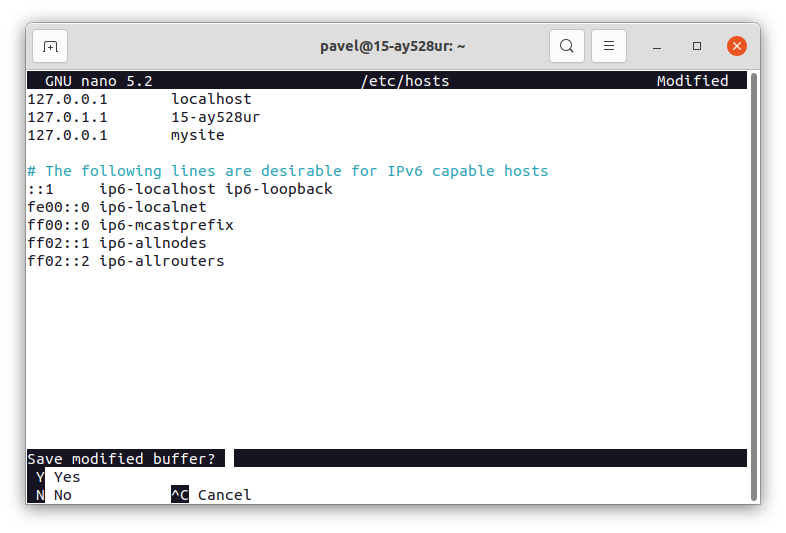
\includegraphics[width=10.5cm]{../_input/programDevelopment/makeDomain/sudo-nano-hosts-step-3.png}
    }
    \caption{Нажали клавишу <<Ctrl>> + <<X>>, затем жмём <<Y>>}
    \label{fig:sudo-nano-hosts-step-3}
\end{figure}

\begin{figure}[p]
    \center{
        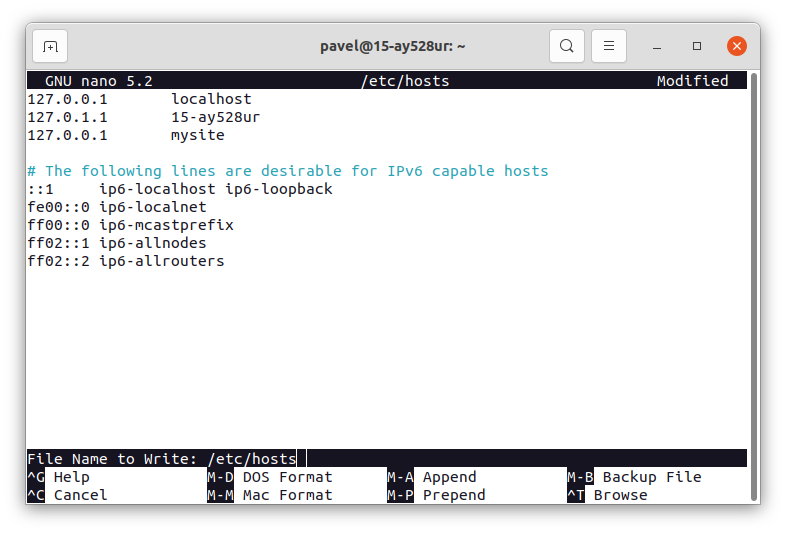
\includegraphics[width=10.5cm]{../_input/programDevelopment/makeDomain/sudo-nano-hosts-step-4.png}
    }
    \caption{Как нажали <<Y>> - жмем <<Enter>>}
    \label{fig:sudo-nano-hosts-step-4}
\end{figure}

Открываем сайт, введя в браузере в адрессной строке <<mysite>>.
Скриншот браузера на рисунке~\ref{fig:browser-mysite} (стр.~\pageref{fig:browser-mysite}).

\begin{figure}[tp]
    \center{
        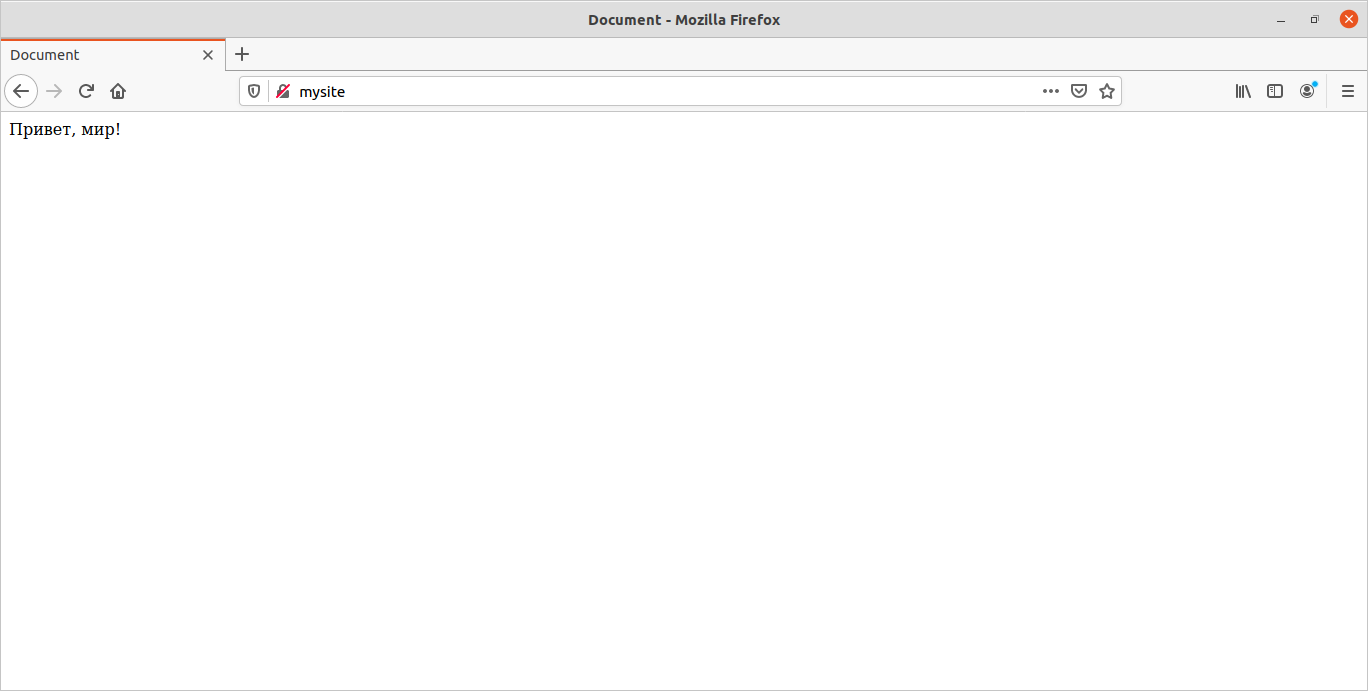
\includegraphics[width=10.5cm]{../_input/programDevelopment/makeDomain/browser-mysite.png}
    }
    \caption{Открыли сайт по домену <<mysite>>}
    \label{fig:browser-mysite}
\end{figure}

\newpage

% = = = = =

\subsubsection*{Запускаем возможность работы файла настроек <<.htaccess>>}

В файле меняем строчку "AllowOverride None" на "AllowOverride All"

\begin{verbatim}
        <Directory /var/www/>
                Options Indexes FollowSymLinks
        #       AllowOverride None
                AllowOverride All
                Require all granted
        </Directory>
\end{verbatim}

Теперь будет работать файл настроек ".htaccess". Создаем файл в директории

\begin{verbatim}
        /var/www/mysite/src
\end{verbatim}

\subsubsection*{Включаем debug mode PHP}

Чтобы отображались ошибки PHP заносим поля:

\begin{verbatim}
        php_flag display_startup_errors on
        php_flag display_errors on
        php_flag html_errors on
\end{verbatim}

\newpage

% = = = = =

\subsection{Разработка модулей}

\textbf{Использованы модули-HTML}
\begin{enumerate}
    \item formInner - модуль, который содержит разметку формы
    \item header - модуль, который сожержит навигацию по сайту
    \item menu - модуль, который содержит HTML разметку меню
\end{enumerate}

\textbf{Использованы модули-PHP}
\begin{itemize}
    \item addElement - модуль, который посылает запрос на создание элемента
    \item connect - модуль, который создает соединение SQL
    \item createTable - модуль, который посылает запрос на создание таблицы
    \item deleteElement - модуль, который посылает запрос на удаление элемента
    \item deleteTable - модуль, который посылает запрос на удаление таблицы
    \item editElement - модуль, который посылает запрос на редактирование элемента
    \item getArrayFromDB - модуль, который получает данные из базы данных в массив
    \item saveCSV - модуль, который на основе массива создает CSV файл
    \item search - модуль, который ищет элементы в массиве и возвращает новый массив
\end{itemize}

\newpage